\section{Results}
\subsection{Networks of partial correlations}
Using the same protocol for calcium signal acquisition  and stimulus presentations as described in Chapter 2, we estimated the noise correlation structure in the superficial layers of visual cortex in 11 scans from 4 mice with PV+ interneurons genetically labeled with a red fluorescent marker.
Each site contained 7--17 interneurons or 2\%--10.3\% of the recorded cells.  
However, these may not be unbiased estimates of the fractions of PV+ neurons because imaged sites were chosen while PV+ cells were  visible.

The recorded population sizes in these sites range from 137 neurons to 385 with the mean of 217. 
As before, the data were binned in 150 ms intervals aligned on stimulus trial onsets; conventional partial correlations matrices were computed and regularized partial correlation matrices were were estimated as described in Chapter 2.
As before, the partial correlation matrix estimates comprised a sparse pairwise component and a low-rank latent unit component.
The sparse component connectivities of 6.9\%--26.8\% (mean 14.8\%) and the number of latent units varied between 39 and 88 (mean 62.3).

Figure \ref{fig:pv1} depicts the sparse component connectivity for three of the eleven sites. 
\begin{figure}
\begin{leftfullpage}
\caption[Examples of functional connectivity in populations with labeled PV+ interneurons]{
{\bf Examples of functional connectivity in populations with labeled PV+ interneurons}

{\bf A.} Populations neurons in superficial layers of visual cortex from three mice. 
The connectivity plot is generated using the same algorithm and color codes as in Fig.~\ref{fig:3}D and \ref{fig:5}G.
The edges between nodes indicate the sparse component of the partial correlation matrix.
The latent units and correlations induced by them are not shown.

{\bf B.} The PV+ neurons and the sparse partial correlations between them in the same imaged sites.
}\label{fig:pv1}
\end{leftfullpage}
\end{figure}

\begin{figure}
\begin{fullpage}
\begin{center}
    \includegraphics[width=\textwidth]{./figures/pv-fig1.pdf}
\end{center}
\end{fullpage}
\end{figure}




\subsection{Functional connectivities by cell pair type}

\begin{figure}
\begin{leftfullpage}
\caption[Functional connectivities for PV--/--, PV--/+, and PV+/+ cell pairs]
{{\bf Functional connectivities for PV--/--, PV--/+, and PV+/+ cell pairs}

Top panels (A,C, and E) show aspects of functional connectivity expressed through conventional noise correlations. 
Bottom panels (B, D, and F) show connectivity expressed through regularized partial noise correlations.
Data points represent averages for each of $n=11$ sites conditioned on cell pair type.
Overall, partial noise correlations provide stronger effects and greater discriminability of cell pair types.

{\bf A.} Average noise correlations. 

{\bf B.} Average partial noise correlations.   

{\bf C.} Rates of positive (green) and (negative) connectivity obtained by thresholding the correlations to make a sparse matrix of interactions.  
The sparsities was matched to matrices in panel D.

{\bf D.} Rates of positive (green) and (negative) connectivity in the sparse component of the partial correlation estimates.

{\bf E.} The ratios of positive connectivity rates to negative connectivity rates based on  thresholded correlations.

{\bf F.} The ratios of positive  connectivity rates to negative connectivity rates based on the sparse component of partial correlation estimates.

}\label{fig:pv2}
\end{leftfullpage}
\end{figure}

\begin{figure}
\begin{fullpage}
\begin{center}
    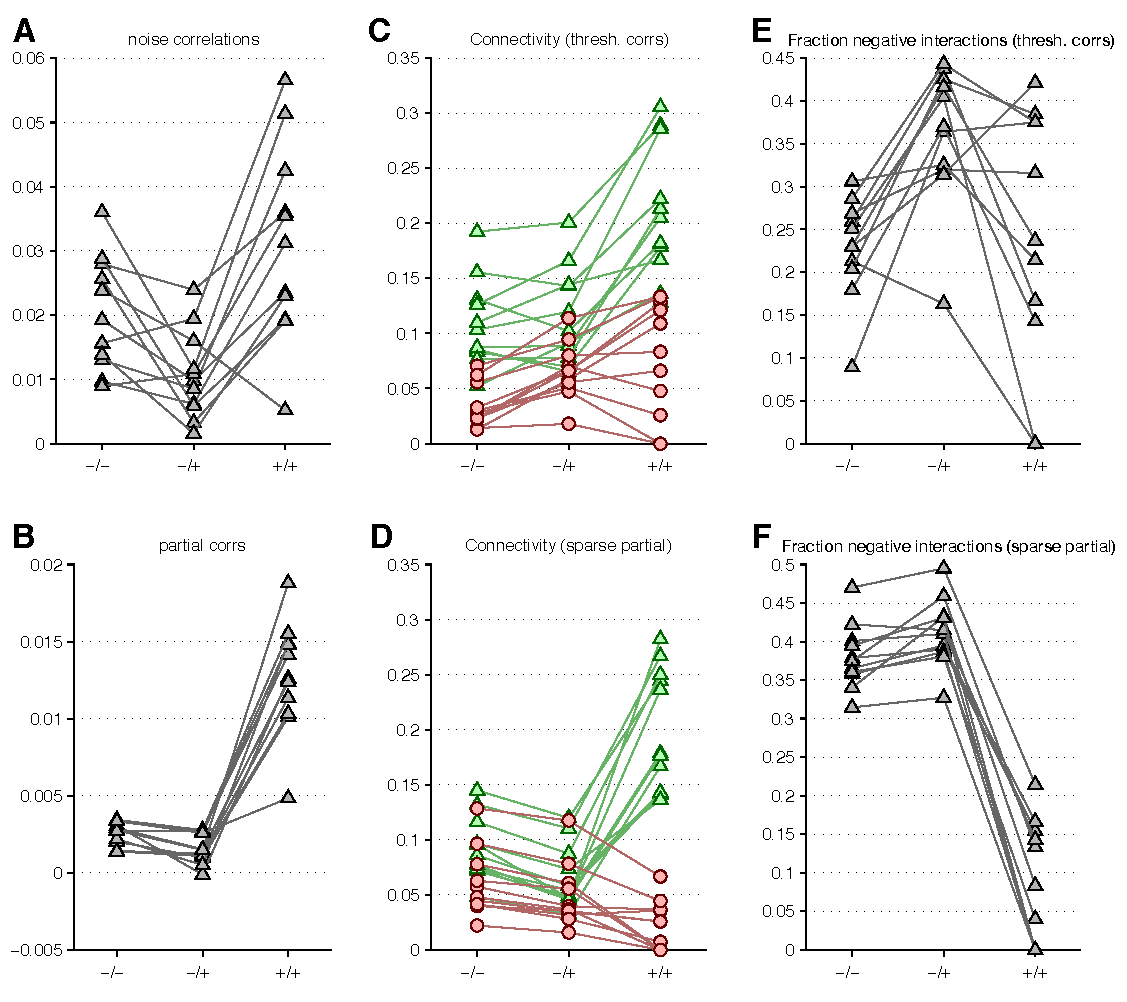
\includegraphics[width=\textwidth]{./figures/pv-fig2.pdf}
\end{center}
\end{fullpage}
\end{figure}

Next, we compared average correlations for both conventional noise correlations and regularized partial correlation matrices conditioned on the cell pair type: 
non-PV to non-PV (--/--), non-PV to PV (--/+), PV to PV (+/+)  (Fig.~\ref{fig:pv2} A and B).
Consistent with \cite{Hofer:2011}, PV+/+ pairs had highest mean noise correlations. The mean +/+ noise correlations were $\times 1.54$ higher than --/-- in unpaired comparisons, but with $n=11$ sites this difference did not reach significance (p=0.08, signed-rank test) due to variability between sites. Both +/+ and --/-- where significantly higher than --/+: Mean +/+ noise correlations were $\times 2.9$ higher than +/-- on average (p=0.003) whereas --/-- noise correlations were $\times 1.9$ higher than --/+.

Similar to our results in the Chapter 2, regularized partial correlations  were lower and most consistent (less dispersed) across sites than sample correlations (Fig.~\ref{fig:pv2} B).
More importantly, the cell pair types were better differentiated with partial noise correlations: 
The average +/+ partial correlations were $\times 4.9$ higher than --/-- and $\times 8.1$ higher than --/+.  
All comparisons were significant (p<0.001, signed rank).
In the language of detection theory, noise correlations differentiated  +/+ site averages from --/-- and --/+ site averages with d-prime values of 0.88 and 1.7, respectively. The partial noise correlations yielded much higher respective d-prime values of 3.8 and 4.2. 

To examine the connectivity rates (connection probabilities) in the sparse network of significant correlations, the noise correlations were thresholded to match the sparsity of the sparse component of the  partial correlation matrix estimates (Fig.~\ref{fig:pv2} C and D). 
Regularized partial correlation estimates provided clearer distinction between the cell pair types yielding consistent relationships between the cell pair types (Fig.~\ref{fig:pv2} D). PV+/+ pairs had severalfold higher rates of positive connectivity ($\times 3.1$ higher than --/+ and $\times 2.2$ higher than --/--. PV--/-- pairs also had the lowest rates of negative connectivity ($\times 2.2$ lower than --/+ and $\times 2.7$ lower than --/+). Notably, --/-- pairs had higher rates of positive and negative connectivity than --/+ pairs, but the ratio of negative connection rates to positive connection rates was highest for --/+ pairs (Fig.~\ref{fig:pv2} F).   All these effects were nearly perfectly consistent between the eleven sites when using partial correlation matrix estimates, yielding signed-rank test p<0.001 even with this small sample size.

Thresholded noise correlations provided much less consistent results with smaller effect sizes (Fig.~\ref{fig:pv2} C and E).

\subsection{Distance dependence of functional connectivity by cell pair type}
We also compared how functional connectivity depended on the distance between cell soma for each cell pair type (Fig.~\ref{fig:pv3}). 
\begin{figure}
\begin{fullpage}
\begin{center}
    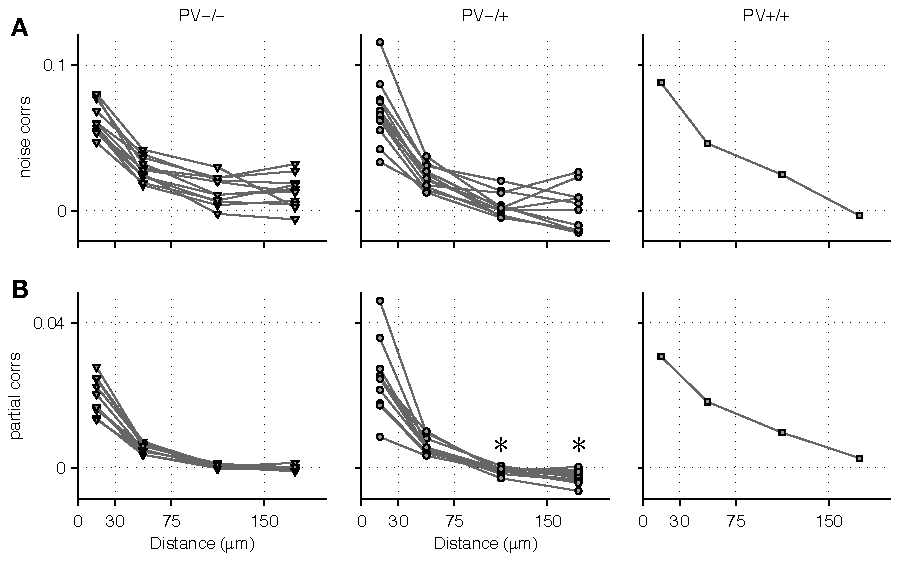
\includegraphics[width=\textwidth]{./figures/pv-fig3.pdf}
\end{center}
\caption[Distance dependence of functional connectivity by cell pair type]
{{\bf Distance dependence of functional connectivity by cell pair type}

{\bf A.} Average noise correlations binned by distance in 11 sites for PV--/-- cell pairs (left), PV--/+ cell pairs (middle), and PV+/+ cell pairs (right, pooled from  all sites).  

{\bf B.} Average regularized partial noise correlations binned by distance in 11 sites for PV--/-- cell pairs (left), PV--/+ cell pairs (middle), and PV+/+ cell pairs (right, pooled from  all sites).  

}\label{fig:pv3}
\end{fullpage}
\end{figure}

We found that partial noise correlations (Fig.~\ref{fig:pv3} B)  yielded clearer effects with greater consistency across sites than conventional noise correlations (Fig.~\ref{fig:pv3} A). While noise correlations remained high and positive for PV--/-- cell pairs, partial noise correlations quickly decayed to distance, suggesting a shorter range of more direct interactions. Interestingly, PV--/+ cells pairs had high average partial correlations for short distances but for distances greater than 100 $\mu$m became reliably negative (p<0.001), suggesting lateral inhibition by PV cells of non-PV cells in adjacent circuits.

\subsection{Orientation tuning dependence of functional connectivity by cell type}
We also compared how functional connectivity depended on the difference in preferred orientations ($\Delta$ori) between cell pairs of each type (Fig.~\ref{fig:pv4}).
\begin{figure}
\begin{fullpage}
\begin{center}
    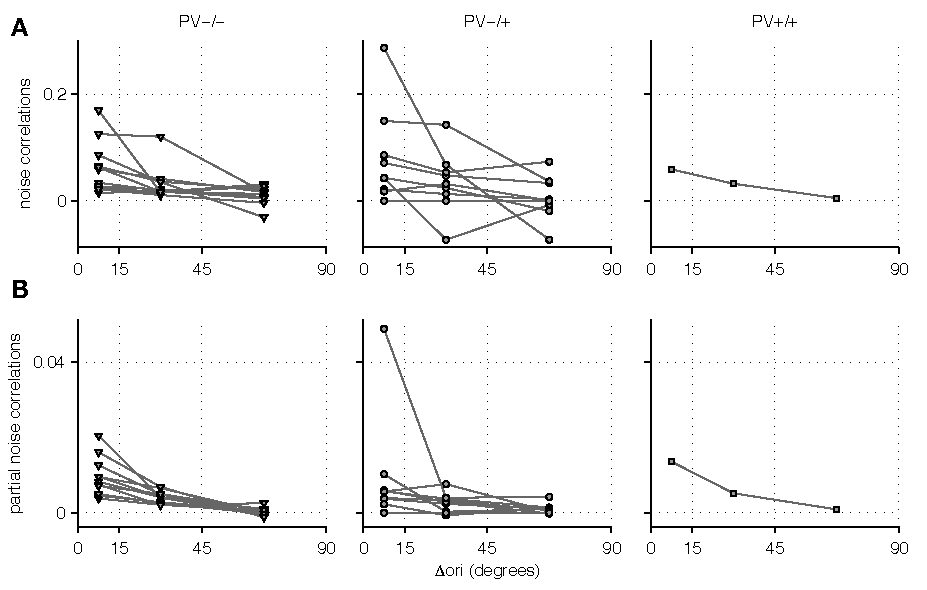
\includegraphics[width=\textwidth]{./figures/pv-fig4.pdf}
\end{center}
\caption[Orientation tuning dependence of functional connectivity by cell pair type]
{{\bf Orientation tuning dependence of functional connectivity by cell pair type}
Each data point represents the average over a site, $n=9$ sites, except for PV+/+ pairs where the data were pooled from all sites.  

{\bf A.} Average noise correlations binned by difference in preferred orientation in 9 sites for PV--/-- cell pairs (left), PV--/+ cell pairs (middle), and PV+/+ cell pairs (right, pooled from  all sites).  

{\bf B.} Average regularized partial noise correlations binned by difference in preferred orientation in 9 sites for PV--/-- cell pairs (left), PV--/+ cell pairs (middle), and PV+/+ cell pairs (right, pooled from  all sites).  

}\label{fig:pv4}
\end{fullpage}
\end{figure}

We found that partial noise correlations (Fig.~\ref{fig:pv4} B) yielded clearer effects with greater consistency across sites than conventional noise correlations (Fig.~\ref{fig:pv4} A).   
Interestingly, partial correlations between PV--/-- pairs were strongly dependent on $\Delta$ori (p<0.04 for both comparisons of adjacent bins) but not between PV--/PV+ pairs. 
This may suggest that while excitatory interactions are sensitive to the single-cell response properties, PV+ cells receive excitatory input less selectively.

